%=====================================================================
% Poster: Replicating SO(2)-Equivariant RL for Closed-Loop Manipulation
% Wade Williams and Joseph Horwitz, CS 5180 (Spring 2026)
%
% Canvas: 36 x 24 in landscape (3:2 ratio), beamerposter, scale 1.05.
% Palette: navy primary, teal accent, cream block body.
% Figures: outputs/plots/learning_curves_combined.pdf and
%          report/figures/env_panel.pdf (both regenerated with the new
%          palette / renderer).
%=====================================================================

\documentclass[final]{beamer}

% 91.44 x 60.96 cm = 36 x 24 in landscape.
\usepackage[orientation=landscape,size=custom,width=91.44,height=60.96,scale=1.05]{beamerposter}
\usetheme{default}
\usecolortheme{default}

% Palatino for a prettier body face; professionalfonts stops beamer from
% overriding it with the default cmss math.
\usepackage[T1]{fontenc}
\usefonttheme{professionalfonts}
\usepackage{mathpazo}

\usepackage{tikz}
\usetikzlibrary{arrows.meta,positioning,calc,shapes.geometric,fit,backgrounds}
\usepackage{booktabs}
\usepackage{amsmath,amssymb}
\usepackage{graphicx}
\usepackage{xcolor}
\usepackage{colortbl}
\usepackage{array}
\usepackage{ragged2e}

%=====================================================================
% Palette
%=====================================================================
\definecolor{Navy}{HTML}{1B2A4E}   % primary -- header bar, block titles
\definecolor{NavyDk}{HTML}{111B33} % darker navy -- footer, rules
\definecolor{Teal}{HTML}{14B8A6}   % accent -- brighter, happier teal
\definecolor{TealLt}{HTML}{CCFBF1} % pale teal -- subtle row highlight
\definecolor{Cream}{HTML}{FFFFFF}  % block body background (now plain white)
\definecolor{Ink}{HTML}{333333}    % body text
\definecolor{Coral}{HTML}{E76F51}  % curve color (RAD in plot)
\definecolor{Sand}{HTML}{E9C46A}   % curve color (DrQ in plot)
\definecolor{Slate}{HTML}{64748B}  % muted baseline
\definecolor{Inv}{HTML}{6C757D}    % invariant-action gray

%=====================================================================
% Block styling -- slim title bar, soft body, no rules
%=====================================================================
\setbeamercolor{block title}{bg=white,fg=Navy}
\setbeamercolor{block body}{bg=white,fg=Ink}
\setbeamerfont{block title}{size=\Large,series=\bfseries}
\setbeamerfont{block body}{size=\normalsize}
\setbeamertemplate{navigation symbols}{}
\setbeamertemplate{itemize item}{\textcolor{Teal}{\textbullet}}
\setbeamertemplate{itemize subitem}{\textcolor{Teal}{--}}
\setbeamertemplate{bibliography item}{}

% Minimal block style: centered Navy title, thin Teal rule, white body.
% Both title and body are beamercolorboxes with explicit leftskip/rightskip
% -- without them, beamer text-sets at frame \textwidth, not columnwidth,
% which caused col 1 body text to bleed into col 2.
\setbeamertemplate{block begin}{
  \par\vspace{0.70cm}
  \begin{beamercolorbox}[wd=\textwidth,sep=0.00cm,leftskip=0.15cm,rightskip=0.15cm]{block title}
    \centering\usebeamerfont*{block title}\insertblocktitle\par
    \vspace{-0.55cm}
    {\color{Teal}\rule{0.98\textwidth}{0.08cm}}
  \end{beamercolorbox}
  \nointerlineskip
  \vspace{-0.30cm}
  \begin{beamercolorbox}[wd=\textwidth,sep=0.00cm,leftskip=0.20cm,rightskip=0.20cm]{block body}
}
\setbeamertemplate{block end}{
  \end{beamercolorbox}
  \vspace{0.25cm}
}

% Beamer blocks default to raggedright; we leave them that way here --
% using \justifying via ragged2e breaks the beamercolorbox rightskip and
% lets body text overflow the column width.

%=====================================================================
% Header / footer bars
%=====================================================================
\setbeamercolor{headbar}{bg=Navy,fg=white}
\setbeamercolor{footbar}{bg=NavyDk,fg=white}

\setbeamertemplate{headline}{
  \leavevmode
  \begin{beamercolorbox}[wd=\paperwidth,sep=1.10cm]{headbar}
    \centering
    \vspace*{0.15cm}
    {\Huge\bfseries SO(2)-Equivariant Reinforcement Learning for Closed-Loop Manipulation\par}
    \vspace{0.30cm}
    {\large Wade Williams \quad\textbullet\quad Joseph Horwitz \quad\textbullet\quad Khoury College of Computer Sciences, Northeastern University \quad\textbullet\quad CS 5180, Spring 2026\par}
    \vspace*{0.05cm}
  \end{beamercolorbox}
}

\setbeamertemplate{footline}{}

%=====================================================================
% Local macros -- consistent equation / label styling
%=====================================================================
\newcommand{\gact}{g\!\cdot\!}
\newcommand{\eq}[1]{\textcolor{Teal}{#1}}
\newcommand{\inv}[1]{\textcolor{Inv}{#1}}

\title{}
\author{}

\begin{document}
\begin{frame}[t]
\vspace*{-0.80cm}

\begin{columns}[t,totalwidth=\textwidth]

\begin{column}{0.005\textwidth}\end{column}

%=====================================================================
% COLUMN 1 -- Problem: motivation, MDP, tasks
%=====================================================================
\begin{column}{0.310\textwidth}
\vspace{0pt}

%--- Motivation: one-paragraph pitch + the four invariance/equivariance rows ---
\begin{block}{Motivation}
Robot manipulation from overhead images has a planar rotation symmetry: rotating the workspace yields an equivalent task with a rotated optimal action. \textbf{Equivariant SAC} encodes this symmetry in the network weights instead of augmenting the training distribution.
\vspace{0.10cm}
\begin{center}\small
\begin{tabular}{@{}rl@{}}
policy equivariance   & $\pi(\gact s) = \gact\pi(s)$ \\[0.10em]
critic invariance     & $Q(\gact s,\gact a) = Q(s,a)$ \\[0.10em]
reward invariance     & $R(\gact s,\gact a) = R(s,a)$ \\[0.10em]
transition invariance & $P(\gact s'\!\mid\!\gact s,\gact a) = P(s'\!\mid\!s,a)$ \\
\end{tabular}
\end{center}
\vspace{0.04cm}
with $g \in C_{8}$, the cyclic group of eight planar rotations (a discretization of $SO(2)$).
\end{block}

%--- Group-invariant MDP: four concise rows, tabular fills full block width ---
\begin{block}{Problem: group-invariant MDP}
\renewcommand{\arraystretch}{1.20}
\begin{tabular}{@{}p{2.4cm}@{\hspace{0.30cm}}p{24.6cm}@{}}
$\mathcal{S}$            & $128\!\times\!128$ depth heightmap concatenated with a tiled scalar gripper-state channel, giving an observation of shape $(2,128,128)$.\\
$\mathcal{A}$            & continuous 5-DoF in $[-1,1]^{5}$, decoded to $(\Delta x,\Delta y,\Delta z,\Delta\theta,a_{\text{grip}})$ with $\Delta_{\text{pos}}=5\,\text{cm}$ and $\Delta_{\text{rot}}=\pi/8$.\\
$\mathcal{P},\mathcal{R}$ & PyBullet rigid-body dynamics; sparse binary reward, $r_{t}{=}1$ on task success and $0$ otherwise.\\
$\gamma,\,H$             & discount $0.99$, horizon $50$ env steps.\\
\end{tabular}
\vspace{0.18cm}

{\small\textbf{Reward invariance.} $R$ is $g$-invariant: $R(\gact s,\gact a) = R(s,a)$ for all $g\in C_{8}$.}

\vspace{0.06cm}
{\small\textbf{Transition invariance.} $P$ is $g$-equivariant: $P(\gact s'\!\mid\!\gact s,\gact a) = P(s'\!\mid\!s,a)$ for all $g\in C_{8}$.}
\end{block}

%--- Experiments: tasks image with (a)(b)(c) labels + symmetry commutative square ---
\begin{block}{Experiments}
\begin{center}
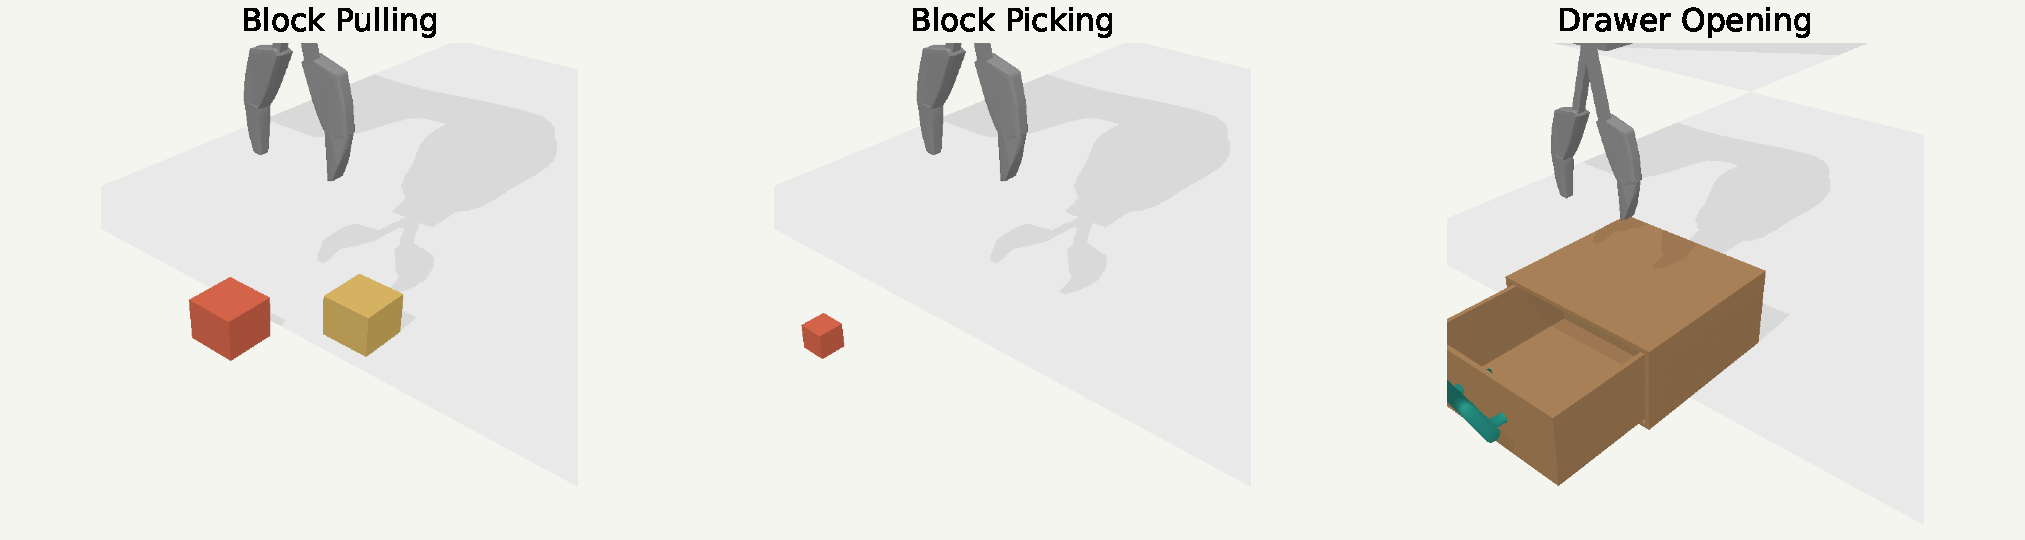
\includegraphics[width=\linewidth]{figures/env_panel.pdf}\\[0.30em]
\makebox[\linewidth]{%
  \parbox{0.33\linewidth}{\centering\small (a) Block Pulling}%
  \parbox{0.33\linewidth}{\centering\small (b) Block Picking}%
  \parbox{0.33\linewidth}{\centering\small (c) Drawer Opening}%
}
\end{center}
\vspace{0.10cm}
{\small Three closed-loop manipulation tasks from the paper: drag a block across the table, pick a block off the table, and open a drawer to a target angle. Same observation, action space, and reward structure in all three.}
\end{block}

\end{column}

\begin{column}{0.020\textwidth}\end{column}

%=====================================================================
% COLUMN 2 -- Method: symmetry diagram, algorithm, architecture
%=====================================================================
\begin{column}{0.335\textwidth}
\vspace{0pt}

%--- Algorithm: standard SAC loop; highlighted line marks the only
%    place the equivariant variant differs from vanilla CNN SAC.
\begin{block}{Equivariant SAC}
\small
\textbf{1.} \eq{Initialize $C_{8}$-equivariant actor $\pi_{\theta}$ and twin critics $Q_{\phi_{1}},Q_{\phi_{2}}$ in \texttt{e2cnn}.}\\[0.20em]
\textbf{2.} Target nets $\bar{\phi}_{i}\!\leftarrow\!\phi_{i}$; warm-start replay $\mathcal{D}$ with scripted expert transitions.\\[0.20em]
\textbf{for} each env step $t=1,\ldots,T$:\\[0.20em]
\hspace*{1em}\textbf{3.} Sample $a_{t}\sim\pi_{\theta}(\cdot\mid s_{t})$, step env, push $(s_{t},a_{t},r_{t},s_{t+1})\to\mathcal{D}$.\\[0.20em]
\hspace*{1em}\textbf{4.} Minibatch $\mathcal{B}\sim\mathcal{D}$; TD target\ $y=r+\gamma\!\left(\min_{i}Q_{\bar{\phi}_{i}}(s',a')-\alpha\log\pi_{\theta}(a'\mid s')\right)$.\\[0.20em]
\hspace*{1em}\textbf{5.} Critic update:\ $\phi_{i}\leftarrow\phi_{i}-\eta\,\nabla_{\phi_{i}}\bigl(Q_{\phi_{i}}(s,a)-y\bigr)^{2}$.\\[0.20em]
\hspace*{1em}\textbf{6.} Actor update:\ $\theta\leftarrow\theta+\eta\,\nabla_{\theta}\!\bigl(\min_{i}Q_{\phi_{i}}(s,a)-\alpha\log\pi_{\theta}(a\mid s)\bigr)$.\\[0.20em]
\hspace*{1em}\textbf{7.} Temperature:\ tune $\alpha$ toward target entropy $\bar{\mathcal{H}}=-|\mathcal{A}|$.\\[0.20em]
\hspace*{1em}\textbf{8.} Polyak:\ $\bar{\phi}_{i}\leftarrow\tau\phi_{i}+(1-\tau)\bar{\phi}_{i}$.
\normalsize
\vspace{0.10cm}
{\small Only \textcolor{Teal}{\textbf{line 1}} changes between Equi SAC and vanilla CNN SAC. Every loss, target, and update rule is standard SAC (Haarnoja et al., 2018); the symmetry lives in the layers.}
\end{block}

%--- Architecture + hyperparameters: all numbers from configs/ ---
\begin{block}{Architecture and hyperparameters}
\small
\textbf{Encoder.} Seven-block $C_{8}$-equivariant CNN in \texttt{e2cnn} (\texttt{R2Conv}, $gspace{=}\mathrm{Rot2dOnR2}(N{=}8)$). Input uses the \emph{trivial representation} (depth and gripper channels are scalars under rotation); hidden layers use the \emph{regular representation}.

\textbf{Actor head.} Final $1{\times}1$ \texttt{R2Conv} outputs one \textbf{irrep(1)} field for $(\Delta x,\Delta y)$ and eight trivial fields for the three invariant action means $(a_{\text{grip}},\Delta z,\Delta\theta)$ plus five log-std parameters.

\textbf{Critic head.} Twin heads each wrap the action as $\text{irrep}(1){\oplus}\text{trivial}^{3}$, mix it into the state feature map with a $1{\times}1$ \texttt{R2Conv}, and pool to a single $C_{8}$-invariant scalar.

\vspace{0.20cm}
\renewcommand{\arraystretch}{1.15}
\begin{tabular}{@{}l@{\hspace{0.6em}}l@{\hspace{1.5em}}l@{\hspace{0.6em}}l@{}}
group                & $C_{8}$              & $\gamma$             & $0.99$         \\
hidden width         & $128$                & $\tau$               & $0.005$        \\
batch size           & $64$                 & learning rate        & $10^{-3}$      \\
replay buffer        & $100\text{k}$        & $\alpha$ (init)      & $0.1$, learned \\
warmup transitions   & $1\text{k}$ expert   & target entropy       & $-5$           \\
env steps / run      & $20\text{k}$         & eval every           & $500$ steps    \\
eval episodes        & $5$                  & seeds per cell       & $2$            \\
\end{tabular}
\end{block}

%--- Symmetry: commutative square showing actor equivariance ---
\begin{block}{Symmetry}
{\small The planar action component $(\Delta x,\Delta y)$ transforms with the world under a rotation $g$; the remaining components $(\Delta z,\Delta\theta,a_{\text{grip}})$ are unchanged. The actor commutes with $g$, the critic is invariant to it.}
\vspace{0.14cm}
\begin{center}
\begin{tikzpicture}[scale=0.46,transform shape,font=\small,>=Stealth,thick]
  \node[draw,line width=1.0pt,fill=white,minimum size=2.4cm,label={[font=\small]above:state $s$}]    (s)  at (0,0) {};
  \begin{scope}[shift={(s.center)},rotate=20]
    \filldraw[fill=Teal!55,draw=Teal,line width=1.0pt] (-0.48,-0.48) rectangle (0.48,0.48);
  \end{scope}
  \node[draw,line width=1.0pt,fill=white,minimum size=2.4cm,label={[font=\small]above:$\gact s$}] (gs) at (6.8,0) {};
  \begin{scope}[shift={(gs.center)},rotate=80]
    \filldraw[fill=Teal!55,draw=Teal,line width=1.0pt] (-0.48,-0.48) rectangle (0.48,0.48);
  \end{scope}
  \node[draw,line width=1.0pt,fill=white,minimum size=2.4cm,label={[font=\small]below:$\pi_\theta(s)$}] (a) at (0,-4.2) {};
  \draw[->,line width=1.8pt,Teal] ($(a.center)+(-0.7,0)$) -- ($(a.center)+(0.7,0)$);
  \node[draw,line width=1.0pt,fill=white,minimum size=2.4cm,label={[font=\small]below:$\gact\pi_\theta(s)$}] (ga) at (6.8,-4.2) {};
  \draw[->,line width=1.8pt,Teal] ($(ga.center)+({-0.7*cos(60)},{-0.7*sin(60)})$) -- ($(ga.center)+({0.7*cos(60)},{0.7*sin(60)})$);
  \draw[->,line width=1.1pt] (s)  -- node[above,font=\small]{$g$} (gs);
  \draw[->,line width=1.1pt] (a)  -- node[above,font=\small]{$g$} (ga);
  \draw[->,line width=1.1pt] (s)  -- node[left,font=\small] {$\pi_\theta$} (a);
  \draw[->,line width=1.1pt] (gs) -- node[right,font=\small]{$\pi_\theta$} (ga);
\end{tikzpicture}
\end{center}
\vspace{0.04cm}
{\small The square commutes by construction: it is enforced in the weights rather than learned from rotated samples.}
\end{block}

\end{column}

\begin{column}{0.020\textwidth}\end{column}

%=====================================================================
% COLUMN 3 -- Results: curves, table, analysis, limits, refs
%=====================================================================
\begin{column}{0.305\textwidth}
\vspace{0pt}

%--- Results: curves + final-checkpoint table in one block ---
\begin{block}{Results}
\begin{center}
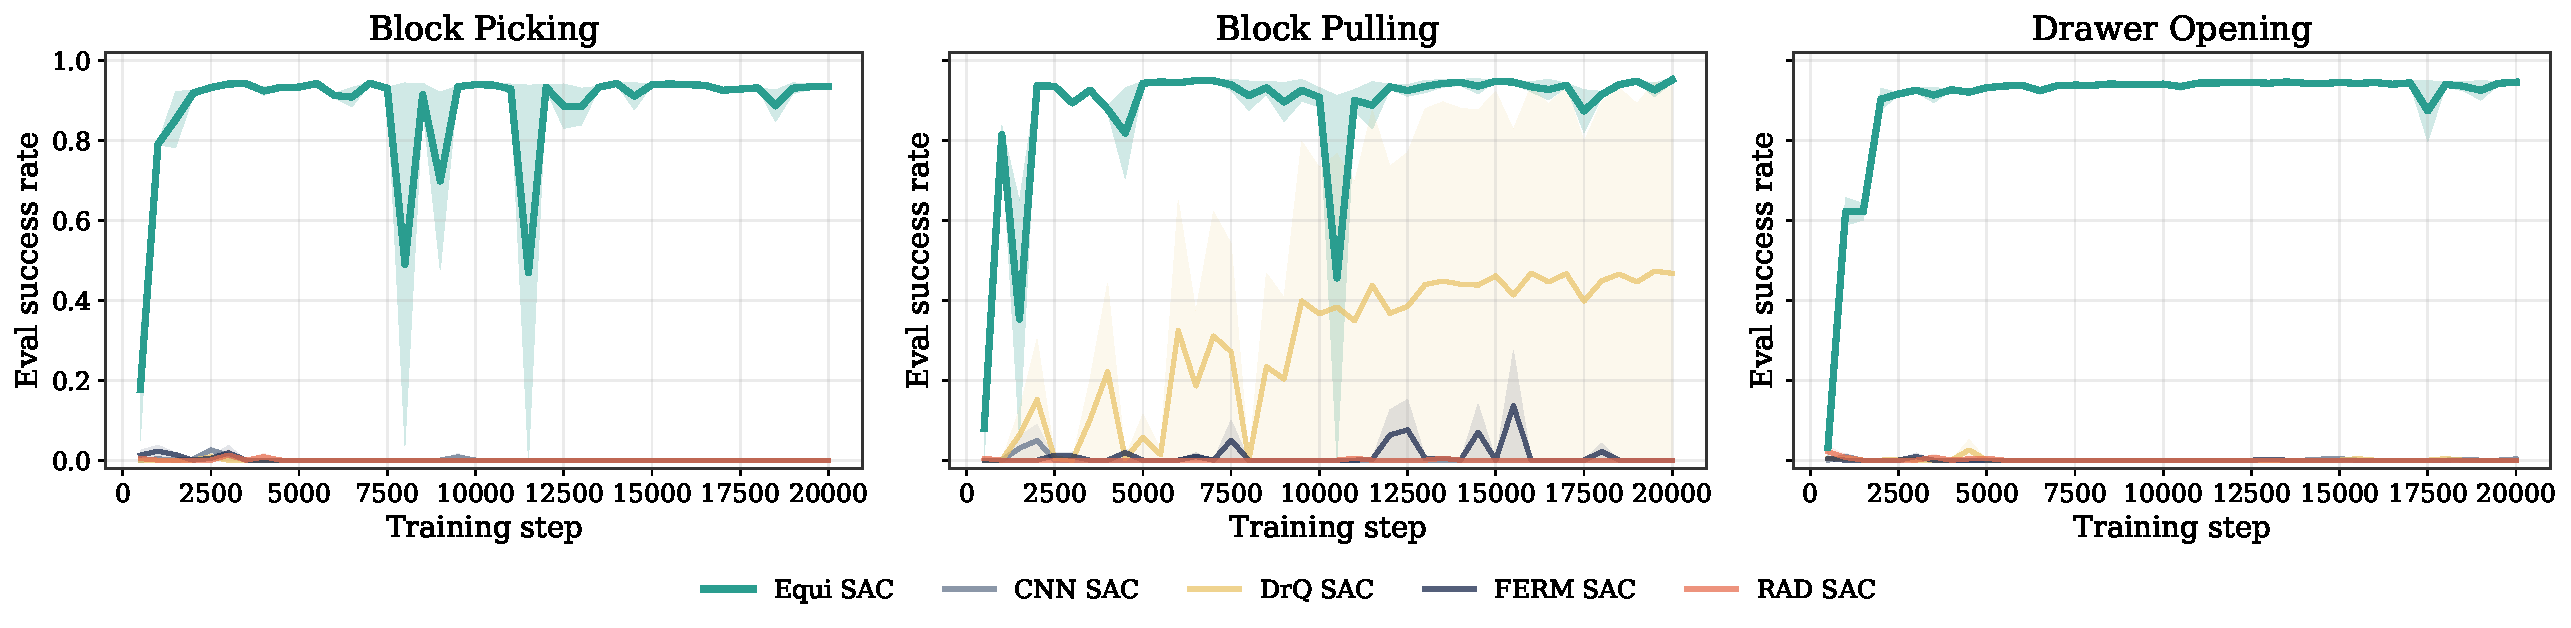
\includegraphics[width=\linewidth]{../outputs/plots/learning_curves_combined.pdf}
\end{center}
{\small Eval success rate vs.\ environment step, mean $\pm 1\sigma$ over $n{=}2$ seeds. Equi SAC (teal) is the only method that solves every task within the 20k-step budget.}

\vspace{0.22cm}
\begin{center}
\footnotesize
\renewcommand{\arraystretch}{1.10}
\begin{tabular}{@{}lccc@{}}
\toprule
                  & \textbf{Pulling} & \textbf{Picking} & \textbf{Drawer} \\
\midrule
CNN SAC           & $0.000$          & $0.000$          & $0.001$         \\
RAD SAC           & $0.000$          & $0.000$          & $0.000$         \\
FERM SAC          & $0.004$          & $0.000$          & $0.000$         \\
DrQ SAC           & $0.460$          & $0.000$          & $0.001$         \\
\rowcolor{Teal!22}\textcolor{NavyDk}{\textbf{Equi SAC}}
                  & $\mathbf{0.936}$ & $\mathbf{0.923}$ & $\mathbf{0.938}$ \\
\bottomrule
\end{tabular}
\end{center}
\vspace{0.05cm}
{\small Mean eval success over the last five checkpoints (training steps 18k--20k).}
\end{block}

%--- Analysis: three tight bullets grounded in the curves ---
\begin{block}{Analysis}
\small
\begin{itemize}
  \item \textbf{Sample efficiency.} Equi SAC reaches ${\sim}0.93$ on every task in \textbf{5k--8k} env steps; no baseline gets off the floor within 20k.
  \item \textbf{Architectural vs.\ statistical equivariance.} DrQ, RAD, and FERM try to learn rotational robustness from augmented views. At this data budget they never find the symmetry; Equi SAC has it from step 0.
  \item \textbf{DrQ on \textsc{block pulling}.} One seed climbs to ${\sim}0.92$, the other stays near 0. The $0.460\pm0.460$ band is seed variance between a success and a failure, not a half-learned policy.
\end{itemize}
\end{block}

%--- Limitations + plan to finish: honest, not hype ---
\begin{block}{Limitations and next steps}
\small
\begin{itemize}
  \item \textbf{Two seeds per cell.} The $0.93$-vs-$0.00$ gap is well beyond seed noise, but $n{=}2$ cannot rank the baselines against each other.
  \item \textbf{Replication, no extension yet.} We reproduce the ranking Wang et al.\ report (Equi SAC clears every task, CNN/augmentation baselines stall) on three tasks with two seeds each; generalization to unseen orientations is not tested.
  \item \textbf{Equivariant DQN is next.} The dispatcher supports \texttt{(alg=dqn,model=equi)}; a CNN-DQN baseline and the DQN trainer still need to run. Omitted here to avoid fabricated curves.
  \item \textbf{Group extensions.} Moving from $C_{8}$ to $D_{4}$ or continuous $SO(2)$ is a small architectural change in the \texttt{e2cnn} \texttt{gspace}.
\end{itemize}
\end{block}

%--- References: compact; scriptsize keeps the block flush in col 3 ---
\begin{block}{References}
\scriptsize
Wang, D., Walters, R., \& Platt, R.\ \emph{SO(2)-Equivariant Reinforcement Learning.} ICLR 2022.\\[0.10em]
Haarnoja, T., Zhou, A., Abbeel, P., \& Levine, S.\ \emph{Soft Actor--Critic.} ICML 2018.\\[0.10em]
Weiler, M., \& Cesa, G.\ \emph{General $E(2)$-Equivariant Steerable CNNs.} NeurIPS 2019.\\[0.10em]
Kostrikov, I.\ et al.\ \emph{DrQ: Image Augmentation Is All You Need.} arXiv:2004.13649, 2020.\\[0.10em]
Laskin, M.\ et al.\ \emph{RAD: Reinforcement Learning with Augmented Data.} NeurIPS 2020.\\[0.10em]
Zhan, A.\ et al.\ \emph{FERM: Efficient Robotic Manipulation.} arXiv:2012.07975, 2020.
\end{block}

\end{column}

\begin{column}{0.005\textwidth}\end{column}

\end{columns}
\end{frame}
\end{document}
